\documentclass[../main.tex]{subfiles}
\graphicspath{{\subfix{../images/}}}


\begin{document}
Python
\subsection{Libraries used}

Keras

Tensorflow (GPU)

Pandas

Numpy

Geopandas

Packages and programming language used.


\subsection{Data pre processing}

The years 2009 through 2018 is chosen to train and evaluate the model. All these files total approximately 130 gigabytes, which will introduce some limitation on how much of the data is processed at once. The process of finding possible routes in this raw data for further processing and validation involves finding all vessels that have visited the port of interest. Due to the file sizes and amount of data for each file this process has to be split into smaller chunks of time windows, \textit{i.e.} the number of consecutive months read in at once and processed. Due too the possibility of vessels starting a route at the end of a month but arriving the first day of the next month, larger time windows are preferred but limitations with memory limit this. Splitting the year into quarters proved to be a good compromise.

First step involves finding which vessels have visited the port of interest, the port of Naantali, for each month. This step is quite computationally time consuming, since every row in each file has to be checked, except rows of a previously known vessel. Only once a vessel has been identified to have visited the port of interest it can be skipped, else the row has to be checked. The process involves checking each rows latitude and longitude and whether the point is within the bounding box seen in Figure \ref{fig:FINLI-box}. This process has to be done once for each file, after which the unique identifiers for every vessel can be stored for future use. The raw files containing millions of row of data at average and begin around one gigabyte on file size limits the number of files that can be processed at once. Every month can have more than 30 unique vessels and the whole timeline has to extracted for all vessels.

\begin{figure}[H]
	\centering
	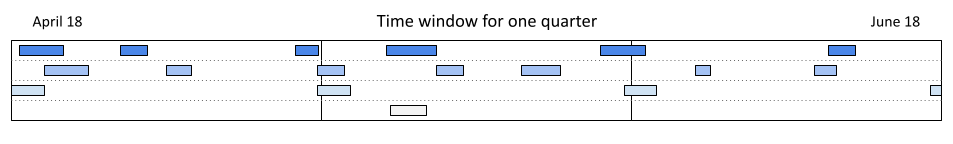
\includegraphics[scale=.45]{timeline.png}
	\caption{Example of one quarter of the the year 2018, a \textit{time window}, and from this time window each unique vessels complete timeline is extracted for further processing. The coloured boxes represents raw AIS data for four unique vessels. Does not represent actual data, rather visualizing the process of finding relevant data in the raw HELCOM dataset.}
	\label{fig:timeline}
\end{figure}

From the complete time window seen in Figure \ref{fig:timeline} only a fraction is used for the final route finding algorithm, see Table \ref{tab:HELCOM-data-percent}. Joining this raw AIS data for every vessel found generates a timeline for each of the unique vessels discovered in the first step.

\subsubsection{Algorithm for extracting routes from dataset}
\label{sec:algo-section}
A route is defined as a series of consecutive AIS messages where the first message in the series is the starting point for a vessel travelling to a port of interest. The last message in the series is the first messages when the vessel has entered the port of interest bounding area, see Figure \ref{fig:FINLI-box}. The routes does not need a specific starting point as this point will be chosen by a set of rules that will define when the route has started. The end of the route will be the same for all vessels as the goal is to find all routes coming from somewhere travelling to the port of interest.

To find routes coming from anywhere and going to a area of interest or port a iterative approach is used. With a complete historical timeline of one vessel, the routes can be discovered by traversing the timeline in reversed chronological order. The end of a route, \textit{i.e.} the start of the search, is the first point where the vessel is leaving the bounding box. From this position traversing the timeline, in reversed chronological order, until a predefined condition is met will give the section of a vessels timeline which equals a route coming from somewhere travelling to a area of interest.

The condition for when the start of the route, end of the search, is met, is whenever the duration of the route has exceeded 48 hours or the vessels speed over ground is zero, standing still, for more than 5 consecutive transmitted messages. The 48 hour time limit was defined for the reason that the maximum travel duration in the Baltic Sea is below 48 hours for a vessel moving at the mean speed and vessels travelling from outside the Baltic Sea has reached Kattegat, approximately, at this time. The reason behind checking that multiple transmitted messages have recorded the speed to be zero is to guarantee that the vessel has actually stopped and not slowed down due to other reasons. This condition can still introduce routes that have not started from another port but will minimize these routes.

\begin{algorithm}[H]
\SetAlgoNoLine
\SetAlgoNoEnd

\SetKwData{Index}{index}\SetKwData{End}{end}\SetKwData{Start}{start}
\SetKwData{Route}{route}\SetKwArray{R}{R}
\KwIn{DataFrame for one vessel sorted in descending time, a \textit{timeline}}
\KwResult{List \R of all routes found}
\emph{The algorithm searches in reverse order of time from reaching the destination until the start of the route}\;
\BlankLine
\ForEach{row in DataFrame}{
	\Index $\leftarrow$ Keep track of current row\;
	\BlankLine
	\If(\tcp*[f]Only true after finding first route){\Route found}{
		\emph{Start searching from first unknown point}\;
		Skip rows until \Index $=$ \Start\;
	}
	\BlankLine
	\If{current point is in PORT}{
		\ForEach{row in DataFrame starting from \Index}{
			\If(\tcp*[f]Vessel is entering the port){point is outside PORT}{
				\End $\leftarrow$ First point reaching the destination\;
				\BlankLine
				\ForEach{row in DataFrame starting from \End}{
					
					\If{start of route reached}{
						\Start $\leftarrow$ Current row\;
						\R $\leftarrow$ Save route from \End to \Start\;
					}
				}
			}
		}
		\tcc{When a route has been found and saved start search again from the last not visited point.}
	}
}
\caption{Find all routes going to a area of interest}
\label{alg:search}
\end{algorithm}
\vspace*{5mm}

Route validation rules were defined to give an efficient way of discarding any routes that would impact the models performance and routes that were off no interest for the scope of the model.

All routes that did not travel for more than eight hours from start to finish were discarded. The reason for this rule comes from the fact that all vessels will be required to travel through the same area for the final part of the voyage, and the model should perform well in this area even though these routes are discarded.

A minimum distance travelled rule was used to discard any routes that travelled less than 200 kilometres, that is the total route distance and not how far away from the port the vessel went. The navigate out from the port of Naantali and the largest bodies of islands outside of Naantali takes approximately 70 kilometres following the fairway.

Any routes that have a time difference between two consecutive AIS messages greater than 12 minutes is also discarded. The reason for this is explained more in details in Section \ref{sec:timeseries}.

Vessels that have returned to the port of Naantali or are returning to the area are also discarded. This combined with the minimum distance travelled required will ensure that for example pilot vessels and other leisure vessels will not be in the final training data. Vessels travelling back to the area are not of interest and will impact the model negatively.

Routes that have faulty data, \textit{i.e.} NaN values or other bad values, and which can not be inferred from the data in any other way is discarded. Examples of this was found where the draught was not recorded only for a small section of the route but could be inferred from the parts where it was recorded. If the values could not be inferred at all the route was discarded completely.

\begin{figure}[H]
	\centering
	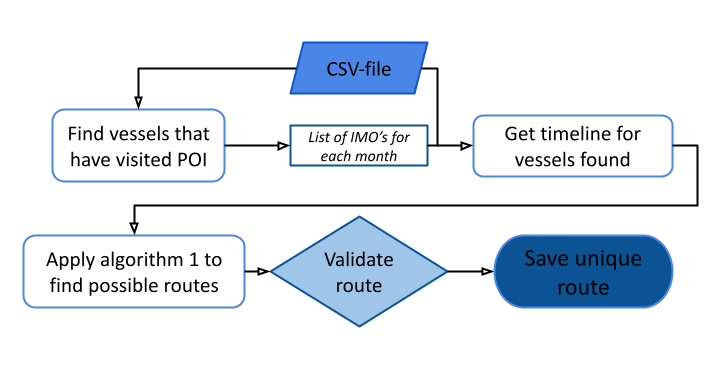
\includegraphics[scale=.5]{data-process.png}
	\caption{Getting routes.}
	\label{fig:flowchart}
\end{figure}

\begin{figure}[H]
	\centering
	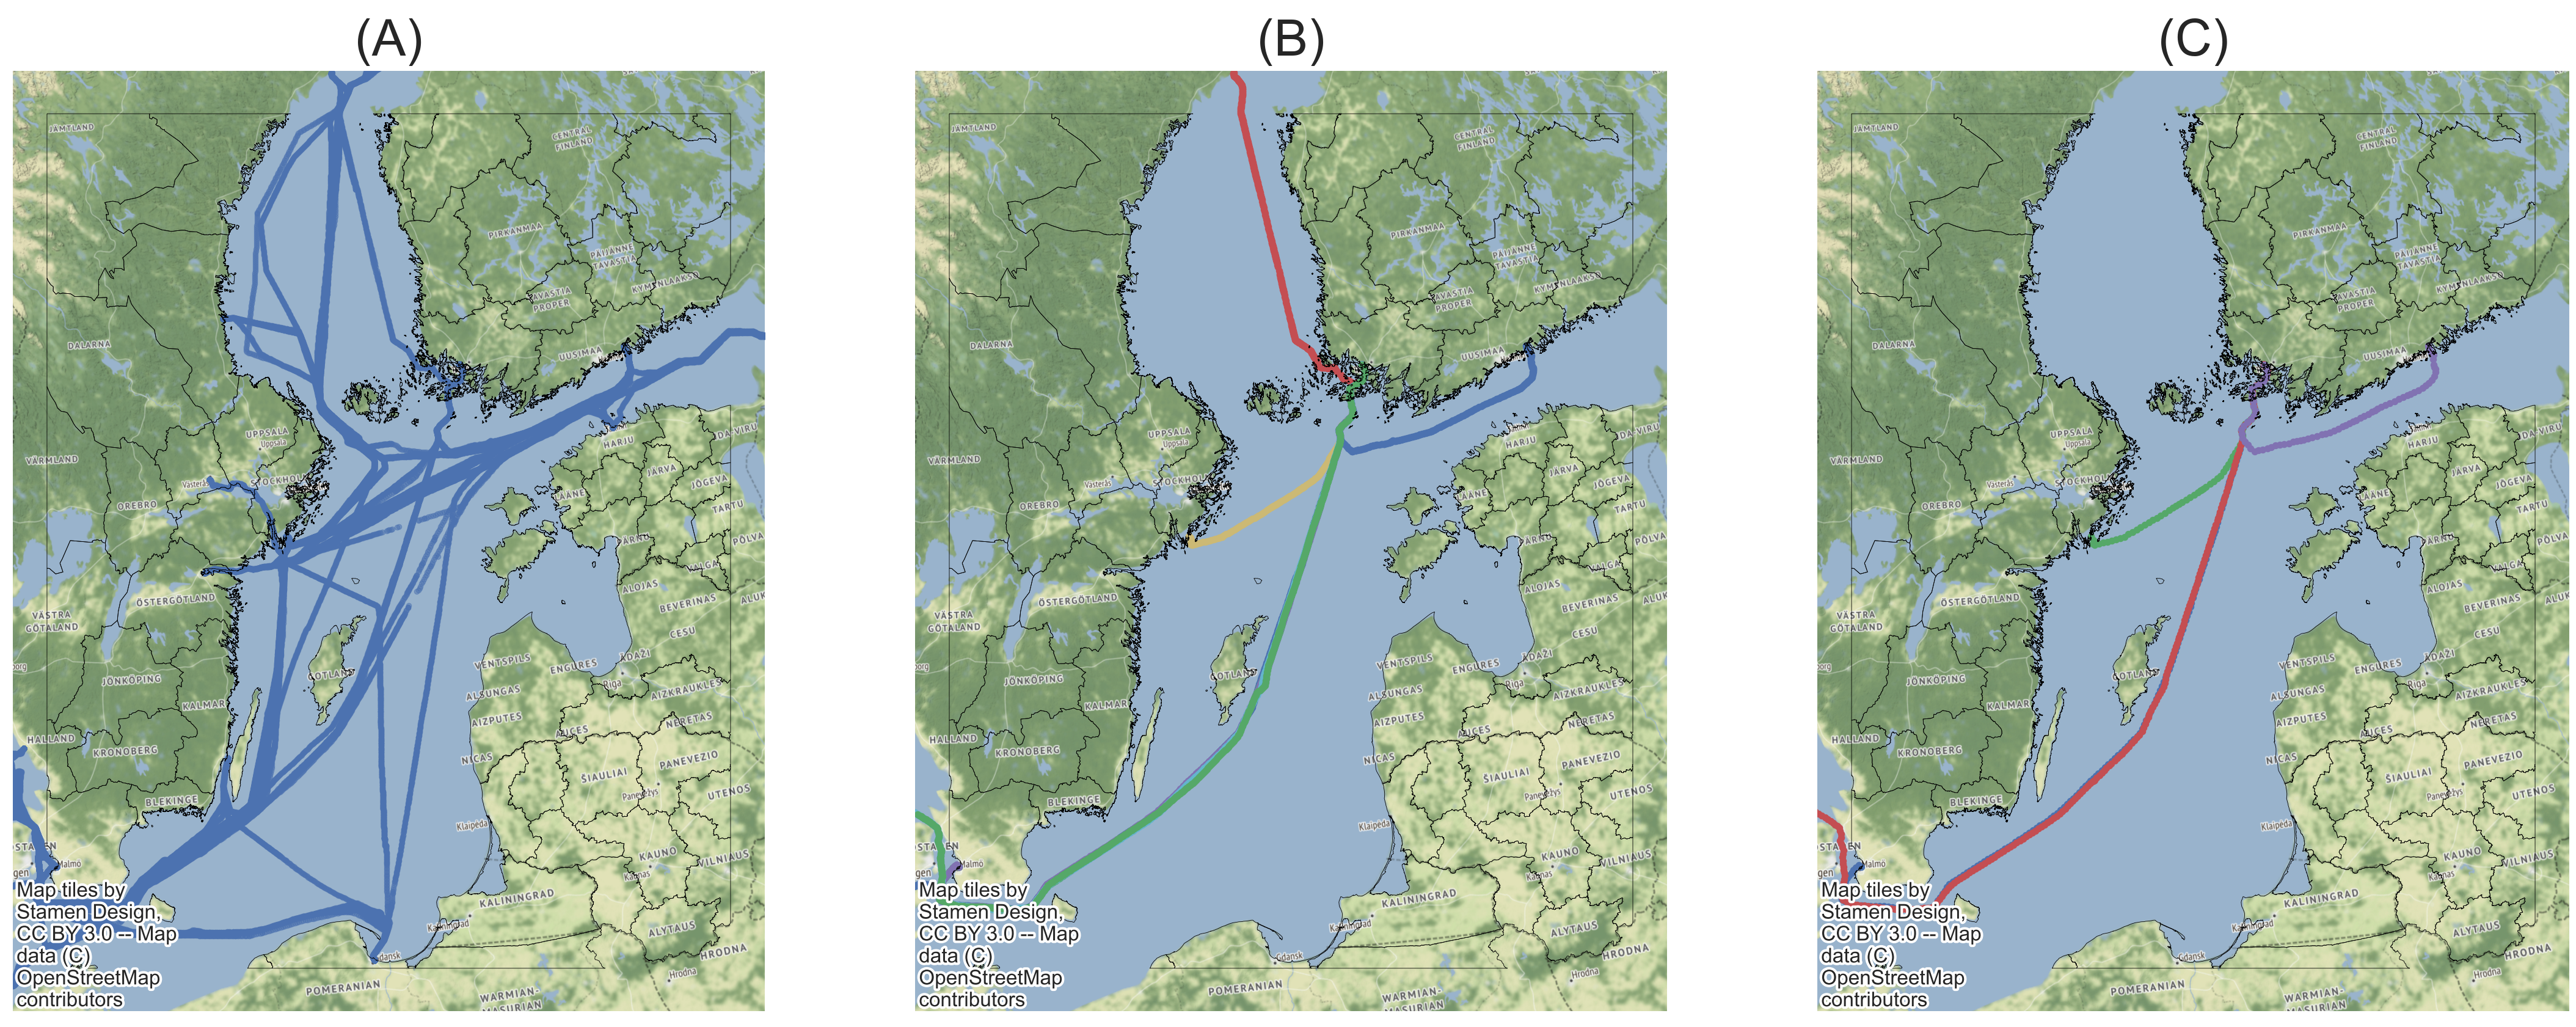
\includegraphics[scale=.45]{route-finding-9256420.png}
	\caption{(A) Complete timeline for one vessel year 2013. (B) All possible routes for the same vessel. (C) All validated routes which are used for training. }
	\label{fig:route-finding}
\end{figure}

The number of routes found from each complete year was at average 1395 routes. 

The total number of routes for the period chosen was 13,955. However, only a fraction of these routes are valid routes. The final route validation and which rules are defined to find viable routes are explained in the next section.
What range of data was used for the final model and reason for so. The problems with AIS data and getting clean routes from start to finish and primarily enough routes for training and testing. 

POI (port of interest could also be thought of as Area of Interest). Timeline is the vessels historical data which is fed into algorithm 1. Route validation according to rules and then save the complete route.

\subsubsection{Coordinate accuracy}

The latitude and longitude recorded in the HELCOM dataset with an accuracy of six decimal places, 0.111 meters, is not necessary.

The level of scaling the coordinate accuracy was chosen to a decimal degree of three places. That will say 0.001 which is 111 meters. The accuracy of the vessels location will be within approximately 100 meters.

\begin{table}[H]
\centering
\begin{tabular}{|l|c|}
\hline
\rowcolor[HTML]{C0C0C0} 
\textbf{Degrees} & \multicolumn{1}{l|}{\cellcolor[HTML]{C0C0C0}\textbf{Distance}} \\ \hline
1.0              & 111 km                                                         \\ \hline
%\rowcolor[HTML]{EFEFEF} 
0.1              & 11.1 km                                                        \\ \hline
0.01             & 1.11 km                                                        \\ \hline
%\rowcolor[HTML]{EFEFEF} 
0.001            & 111 m                                                          \\ \hline
0.0001           & 11.1 m                                                         \\ \hline
%\rowcolor[HTML]{EFEFEF} 
0.00001          & 1.11 m                                                         \\ \hline
0.000001          & 0.111 m                                                         \\ \hline
\end{tabular}
\caption{Coordinate accuracy by decimal places in decimal degrees for latitude and longitude, from \cite{GIS_2011}}
\label{tab:gis-accuracy}
\end{table}

AIS messages transmitted within approximately 100 meters of each other will be thought of as sent from the same location using this scaling level. With a average vessel speed for all routes used, see Figure \ref{fig:sog-dist}, of approximately 14 knots (25 km/h) and a time difference between messages of 10 minutes a vessel will have moved 2.2 nmi (4.1 km) during this time. With a positional accuracy of approximately 100 meters this distance can vary but on the open sea a difference in $\pm$ 100 meters does not impact the overall time it will take to reach the destination.


\subsubsection{Feature selection}

The features chosen for training the model on was decided by what is available in the HELCOM dataset, what is possible to infer from available data and what has been proven to be efficient features by previous studies \cite{El_2020, Jahn_2018}.

Most of the features available in the HELCOM dataset was used for the model; latitude and longitude for the position of the vessel at a given point in time, sog to indicate the vessels moving rate, cog for where the vessels trajectory is heading, draught to indicate the vessels physical capabilities in combination with the vessel class feature, which is a combination of features, see Figure \ref{fig:vessel-class-def} and finally the distance to the destination calculated from the historical route the vessel has taken.

Using the distance left to the destination as a feature does mean that the problem to be solved is in its simplicity learning the time it will take to traverse the distance left at the current speed. However, there are many factors that will impact the time it will take to reach the destination which can not be learned from only the distance to travel and the speed. 

The target to predict is time to destination (\textit{TTD}) which is in minutes. The TTD prediction is added to the current time and thus give an ETA.

\subsubsection{Time series data windowing and time distribution}
\label{sec:timeseries}

With the routes validated a final processing step is required to generate the time series data that is fed to the network. Since regular RNN suffers from poor performance when the data is unevenly sampled in terms of time difference between samples, it is vital to normalize the time difference between time steps. The nature of AIS and the HELCOM dataset means that it is only viable to normalize the sampling interval to a certain degree.

A compromise with the time difference between messages was achieved by as evenly as possible sample data with longer time intervals, discarding messages in that interval, and by this achieving a improved time series with preferable time difference normalization. In this improved time series the difference between messages is on average at most three minutes. A lower limit of nine minutes was chosen to conform with what was discovered in Section \ref{sec:AIS-stat} and \ref{fig:ais-msg-dist} and the upper bound of twelve minutes has been set when validating the routes. On average, two messages will get discarded so the time difference is nine minutes. Shorter time intervals should be possible with raw AIS data, but for the dataset used the number of routes that were viable without generating data between messages were too few. Decreasing the longest allowable gap between AIS messages in a route discarded too many routes, \textit{i.e.} a route with at any point a time difference between messages smaller than twelve minutes would have been rejected.

\begin{figure}[H]
	\centering
	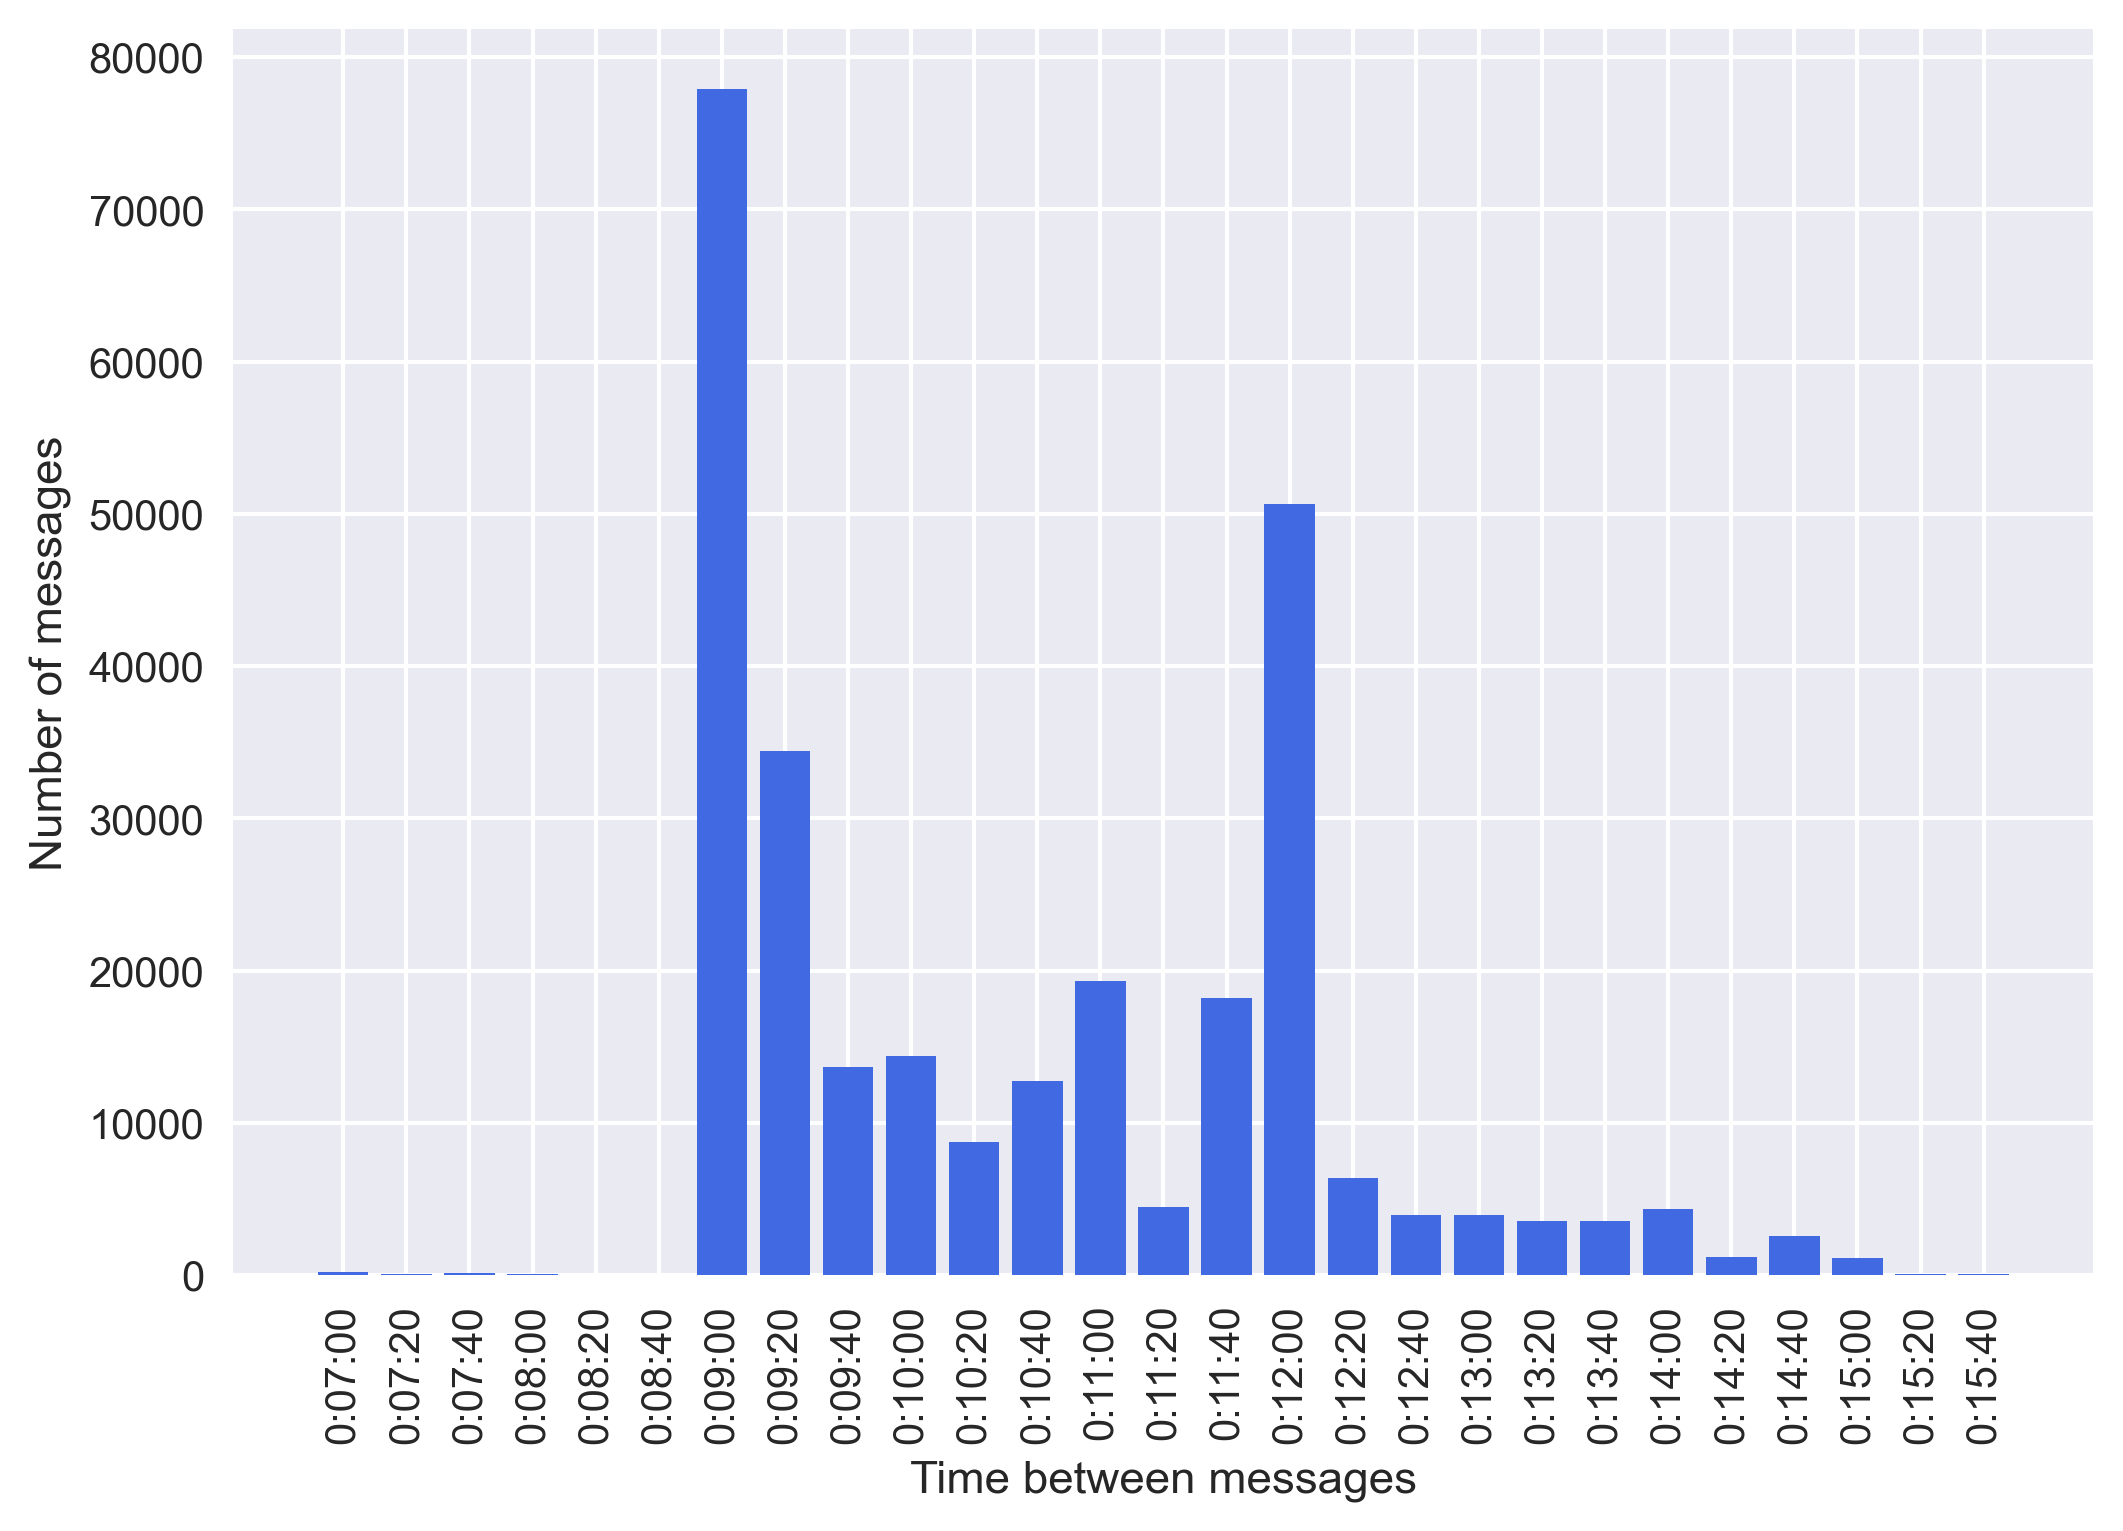
\includegraphics[scale=.6]{2009-2018-routes-message-dist.png}
	\caption{Normalized time differences between messages.}
	\label{fig:norm-time}
\end{figure}

In Figure \ref{fig:norm-time} the normalized time differences are in the range from nine to twelve minutes with only some exceptions that have a time difference shorter than or longer than this range. The exceptions are for the most part due to the inconsistencies in the recorded time intervals, \textit{e.g.} given one message at time zero $t_0$ with the following messages at $t_{+4}$, $t_{+4}$ and $t_{+7}$ (minutes from the previous message) so the two following messages will not be more than nine minutes from the first and the third message will therefore be chosen as the next point in time, with a 15 minute difference. 

\begin{figure}[H]
	\centering
	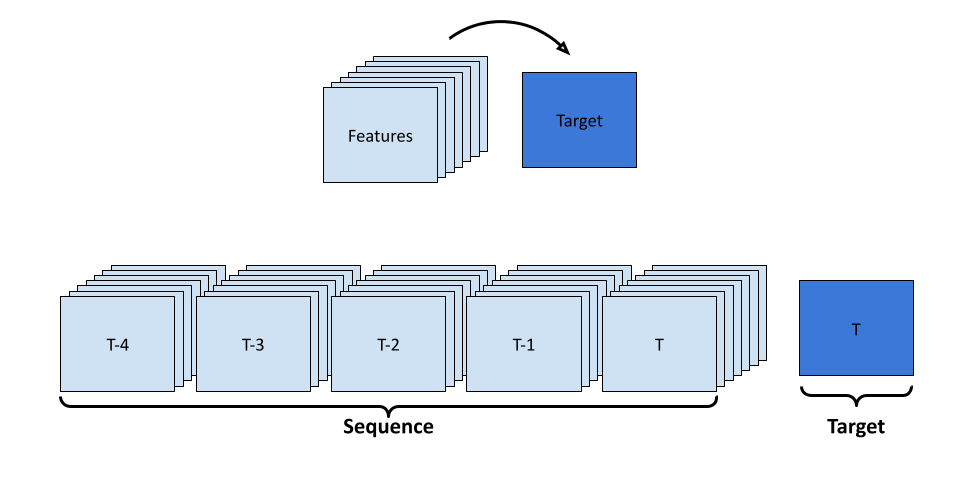
\includegraphics[scale=.4]{sequenced-data.png}
	\caption{Timeseries sequenced data, with a time window width of five. Each timestep in the sequence has a time difference in the range defined.}
	\label{fig:seq-data}
\end{figure}

With a route consisting of AIS messages with a time difference distribution in the range mentioned above a time window of timesteps is generated for the whole route. A time window is defined as $n$ number of consecutive timesteps that create a window of time for the route. Each timestep in this time window consists of all chosen features and the target TTD. For all but the last timestep, the target is discarded and only the final timestep target is set as the target to predict. Sliding the time window over the whole route one timestep at a time generates a set of windows that each covers $n$ timesteps. 

\begin{figure}[H]
	\centering
	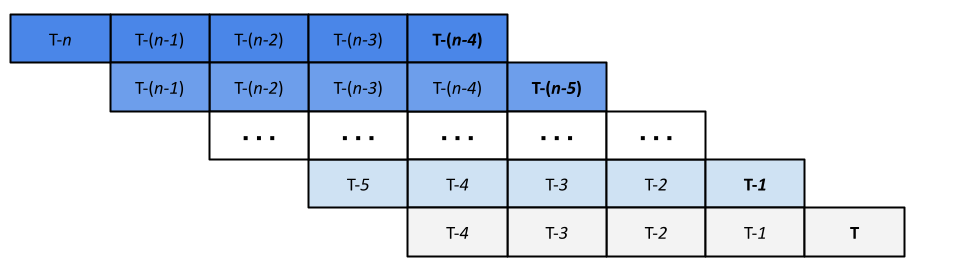
\includegraphics[scale=.4]{time-window.png}
	\caption{Sliding time window for a complete route starting from the end at $T-n$ and ending at the last timestep $T$. A prediction will be made for every last timestep in the time window, marked with bold.}
	\label{fig:time-window}
\end{figure}

A prediction will be made for the last timestep in the time window, which in terms of real time prediction will require that for the first four timesteps, AIS messages received, a prediction can not yet be made. Only after the fifth message can a prediction be made. This also means that any five historical AIS messages could be used, if they fulfil the requirements for the time window.


\subsection{ML model}

Description of the neural network model used and tested to find the optimal performer


\subsection{Comparison model}

!!! If the travel distance left to destination is used in nmi for example, test the accuracy against simply calculating time left by the current speed and distance left 

\end{document}